\documentclass[conference]{IEEEtran}
\IEEEoverridecommandlockouts
\usepackage{cite}
\usepackage{amsmath,amssymb,amsfonts}
\usepackage{algorithmic}
\usepackage{graphicx}
\usepackage{textcomp}
\usepackage{xcolor}
\usepackage{url}
\usepackage{array}
\usepackage{tikz}
\usetikzlibrary{arrows.meta,positioning,fit,calc}
\hyphenpenalty=10000
\exhyphenpenalty=10000
\emergencystretch=1.5em
\raggedbottom
\makeatletter
\newcommand{\authorflushleft}{\end{@IEEEauthorhalign}\hskip 0pt plus -1fill\begin{@IEEEauthorhalign}}
\newcommand{\linebreakand}{\end{@IEEEauthorhalign}\hfill\mbox{}\par\mbox{}\hfill\begin{@IEEEauthorhalign}}
\makeatother
\def\BibTeX{{\rm B\kern-.05em{\sc i\kern-.025em b}\kern-.08em
    T\kern-.1667em\lower.7ex\hbox{E}\kern-.125emX}}

% ---------------------------------------------------------------------
\newcommand{\embmodel}{\texttt{snowflake\allowbreak-arctic\allowbreak-embed\allowbreak-xs}}
\newcommand{\embdim}{384}
\newcommand{\rerankmodel}{\texttt{ms\allowbreak-marco\allowbreak-MiniLM\allowbreak-L\allowbreak-6\allowbreak-v2}}
\newcommand{\llmname}{GPT\nobreakdash-6 Luna}
% ---------------------------------------------------------------------

\tikzset{
  box/.style={draw, rounded corners=2pt, align=center, font=\footnotesize,
              minimum height=6mm, inner sep=3pt, fill=white},
  store/.style={box, fill=gray!12},
  llm/.style={box, fill=gray!28, font=\footnotesize\bfseries},
  arr/.style={-{Stealth[length=2mm]}, semithick},
  grp/.style={draw, dashed, rounded corners=3pt, inner sep=4pt}
}

\begin{document}

\title{E.C.H.O: An Intent Aware Personal Memory System for Unified Search Across Email, Web, and Video History}

\author{\IEEEauthorblockN{1\textsuperscript{st} Arjun Sai N}
\IEEEauthorblockA{\textit{Dept. of Computer Science} \\
\textit{and Engineering} \\
\textit{PES University}\\
Bengaluru, India}
\and
\IEEEauthorblockN{2\textsuperscript{nd} Mohammed Mir Fazlai Ali}
\IEEEauthorblockA{\textit{Dept. of Computer Science} \\
\textit{and Engineering} \\
\textit{PES University}\\
Bengaluru, India}
\and
\IEEEauthorblockN{3\textsuperscript{rd} Mohammed Shehzaad Khan}
\IEEEauthorblockA{\textit{Dept. of Computer Science} \\
\textit{and Engineering} \\
\textit{PES University}\\
Bengaluru, India}
\linebreakand
\IEEEauthorblockN{4\textsuperscript{th} Mrigank Jain}
\IEEEauthorblockA{\textit{Dept. of Computer Science} \\
\textit{and Engineering} \\
\textit{PES University}\\
Bengaluru, India}
\and
\IEEEauthorblockN{5\textsuperscript{th} Mannuru Shalima Sulthana}
\IEEEauthorblockA{\textit{Dept. of Computer Science} \\
\textit{and AIML} \\
\textit{PES University}\\
Bengaluru, India}
}

\maketitle

\begin{abstract}
Take one interview. The invitation sits in Gmail, the articles read to prepare for it sit in Chrome's history, and the tutorials sit in YouTube's watch history. Each app has its own search box, and none of them knows what the other two hold. We built E.C.H.O (Efficient Contextualized History Orchestrator) to fix this for a single user. It brings Gmail, Chrome, and YouTube activity into one store on the user's laptop and answers questions about it in plain language. What gets stored depends on the source. All mail is kept, except what Gmail has already put in spam or trash, but a page or a video is kept only when foreground time, scrolling, watch time, or a return visit shows that the user paid attention to it. A background worker then cleans each item, pulls out the text of its attachments, puts it in one of five broad categories, and embeds it. To answer a question, a language model plans the search, while the search itself is plain code behind a single tool. That tool runs keyword and vector search together, merges the two lists with reciprocal rank fusion, widens the search if the results look weak, and reorders the rest with a local cross encoder. Most questions take two model calls, and the code puts a hard stop at six. The model sees just the question and limited excerpts, not database rows and not the whole store. A wellbeing module shows how time was spent without judging it, and it also files items into the user's own goals automatically only when two signals agree. Everything else waits for the user. We tested E.C.H.O on 119 items (78 emails, 30 pages, and 11 videos) with 38 questions. The first ten results held 93\% of the relevant items, a question needed 2.3 model calls and a median of 8.1 seconds, and the stored items matched the capture rules in all 13 clean scripted sessions. One result went against our design. Semantic search alone ranked better than the full pipeline. In the questions we examined, the cross encoder gave all candidates a score near zero, so the engagement term ended up deciding the order.
\end{abstract}

\begin{IEEEkeywords}
personal information management, retrieval augmented generation, hybrid search, reciprocal rank fusion, tool calling agents, intent aware capture, local first software, digital wellbeing
\end{IEEEkeywords}

% ---------------------------------------------------------------------
\section{Introduction}
% ---------------------------------------------------------------------
Placement season at PES University shows the problem well. A company mails the interview schedule, and over the next few days the preparation spreads out, with operating systems articles in Chrome and a few explanations on YouTube. A week later, right before the interview, all of it is needed again. By then the email is in Gmail, the videos are in the YouTube watch history, and the articles are somewhere in Chrome's history. Each app searches only its own data, so getting everything back means three separate searches and some guessing about which app holds what.

Keeping a record of everything a person has seen is an old idea. Bush described the memex in 1945 \cite{b1}, and much later Stuff I've Seen \cite{b2} and MyLifeBits \cite{b3} built working stores of a person's mail, pages, and documents. Still, it has not become something people use daily, and noise is a big reason for that. A browser logs every page that opens, stray clicks and tabs closed after two seconds included, and a memory built straight on that log is mostly pages nobody read. Our capture test has exactly this case, a page closed after three seconds, and E.C.H.O is expected to drop it (Section~\ref{sec:eval}). And even a clean memory is hard to search. A search box wants the right keyword, but people do not remember keywords. They remember something like ``the OS material I read after the interview email.''

E.C.H.O deals with each problem at a different point. Noise is handled at capture. A page or a video is stored only if engagement shows that the user actually attended to it, so the stray tab does not reach the database at all. The keyword problem is handled at search time. E.C.H.O searches by meaning as well as by keyword, and a language model turns the user's loose phrasing into concrete searches. Mail, pages, and videos share one data model on the user's laptop, they get enriched in the background, and the user asks about them in natural language. Each answer is built from the stored items, following retrieval augmented generation \cite{b4}.

Our work makes four contributions:
\begin{itemize}
\item For capture, a separate set of rules for each source, and privacy filters that act before anything is stored. Sensitive pages lose their text, secret parameters are cut from addresses, and private work apps keep just their page title. The stored items matched these rules in all 13 clean scripted sessions.
\item One local storage model, in which emails, pages, and videos share a central table within a schema of 17 tables. PostgreSQL is the permanent record, Redis holds short lived state, and the FAISS index can be rebuilt from PostgreSQL at any time. Attachment text is pulled out when the mail arrives, which makes a PDF as easy to find as the email it came with.
\item Retrieval through a bounded agentic loop. The language model plans and phrases each search, and a deterministic tool carries it out with hybrid keyword and vector search, rank fusion, a rule based quality check that widens weak searches, and cross encoder reranking. On the test questions, a turn needed 2.34 model calls on average, and the code allows at most six.
\item Finally, a wellbeing module that reports time, sessions, and declared regret in descriptive terms, together with a grouping engine for the user's own goals. An item is filed on its own only when a rule match and a neighbor score of at least 0.85 agree, and one click undoes it. All the other suggestions wait for the user. At 0.85, no item from outside a group got in during our test.
\end{itemize}

After related work in Section~\ref{sec:related} and an overview in Section~\ref{sec:overview}, the design follows in Sections IV to VI, covering capture, storage, enrichment, retrieval, wellbeing, and privacy. Section~\ref{sec:impl} describes how we built it, Sections VIII and IX report the results and their limits, and Section~\ref{sec:conc} concludes.

% ---------------------------------------------------------------------
\section{Related Work}\label{sec:related}
% ---------------------------------------------------------------------
\subsection{Personal Information Management}
Bush pictured the memex as a desk that keeps a person's books, records, and letters and brings any of them back quickly \cite{b1}. Stuff I've Seen put everything a person had already seen, such as an email, a web page, or a document, under one index, and used the fact that the person had seen it before as a cue for search \cite{b2}. MyLifeBits went further and tried to keep everything that could be captured, in a SQL database \cite{b3}. E.C.H.O wants what these systems wanted, which is to help a person find something again. Where it differs is in what it keeps and what it gives back. MyLifeBits would store the page that was open for three seconds, but E.C.H.O never writes it. Stuff I've Seen returns a list of results, while E.C.H.O returns an answer, with a small pill for each source it used.

\subsection{Retrieval Augmented Generation and Tool Use}
In retrieval augmented generation, a retriever fetches documents and a text generator writes its answer from them \cite{b4}. In E.C.H.O, the retriever is the \texttt{search\_memories} tool and the generator is \llmname{}, and the steps are arranged as a graph built with LangGraph \cite{b5}. ReAct showed that a language model can alternate between reasoning and actions such as search calls, and that grounding each step in tool output reduces invented facts \cite{b13}. We borrow this pattern, but in a deliberately narrow form. The model has exactly one read only tool. Apart from two small local encoders, this tool has no model inside it. Also, the code caps how many rounds the model gets.

\subsection{Hybrid Search and Reranking}
Sentence BERT showed that texts can be turned into vectors whose cosine similarity follows their meaning \cite{b6}. E.C.H.O embeds every item with a small local sentence model \cite{b16} and searches the vectors with FAISS \cite{b8}. Keyword search comes from the full text search built into PostgreSQL, and it also catches what meaning misses, such as sender names, domains, and channel names. During testing in July, a question about ``emails from Neon'' could not match the sender at all until we added senders to the text index. The problem is that these two methods score on unrelated scales, so it does not make sense to add their scores directly. Reciprocal rank fusion solves this because it uses just the position of each item in each list \cite{b9}. After fusion, a cross encoder reads the question and a candidate together and scores how well they match. Nogueira and Cho showed that this works well for passage reranking \cite{b10}. Our cross encoder is a compact MiniLM \cite{b7} model, trained on the MS MARCO passage ranking data \cite{b11}.

\subsection{Local First Software}
Kleppmann et al.\ describe local first software, where users own their data and the application works from a copy on their own device \cite{b12}. E.C.H.O follows the same idea, as the database, the vector index, the cache, and both encoders all run on the user's laptop. The hosted language model gets only limited pieces of text.

\subsection{Digital Wellbeing Tools}
Lyngs et al.\ reviewed hundreds of digital self control apps and browser extensions. They found that most of them block, limit, or track usage against a goal \cite{b14}. E.C.H.O leaves the judgment to the user. It shows where the time went, and the user decides which items they regret, with no score and no blocking. We hold the generated text to the same rule. The weekly reflection is checked for judging phrases before it is shown, and if it fails that check, the user sees plain numbers instead (Section~\ref{sec:wba}).

% ---------------------------------------------------------------------
\section{System Overview}\label{sec:overview}
% ---------------------------------------------------------------------
Fig.~\ref{fig:arch} shows the main parts of the system. First, data comes in through three connectors. The Gmail connector reads mail through the Gmail API with OAuth, and it asks only for the changes since its last check. The Chrome extension follows desktop browsing and YouTube playback. It runs on the whole YouTube site and not only on \texttt{/watch} pages. YouTube switches videos without reloading the page, so an earlier version of the extension missed the videos that a user opened from inside the site. The YouTube connector then adds each video's details from the YouTube Data API. Next, all connectors send their items to one FastAPI gateway, and there the storage engine writes each item in a single transaction and skips anything already stored.

The work is then split across three stores. PostgreSQL keeps the permanent record of all items. FAISS keeps the embedding vectors, and we treat it as something that can always be rebuilt. We learned this in July, when a corrupted metadata file left semantic search silently returning nothing, and we rebuilt the index from the text stored in PostgreSQL. Keeping the stored text identical to the embedded text is what makes such a rebuild exact. Redis holds the short lived state, such as revisit flags, cached attachment text, reminder state, and the user's capture settings. All of this runs on the user's laptop.

Three modules work on top of the stores. The enrichment worker (ENP) prepares new items for search in the background. On the six new emails in our test, it needed about 3.1 seconds per item, around 19 items a minute, with PDF text extraction included. The retrieval engine (RSE) answers questions. The wellbeing module (WBA) turns the stored activity into time summaries, sessions, regret patterns, and group suggestions. The user works mainly in a React dashboard, and a small popup in the extension can pause capture at any time.

\begin{figure}[t]
\centering
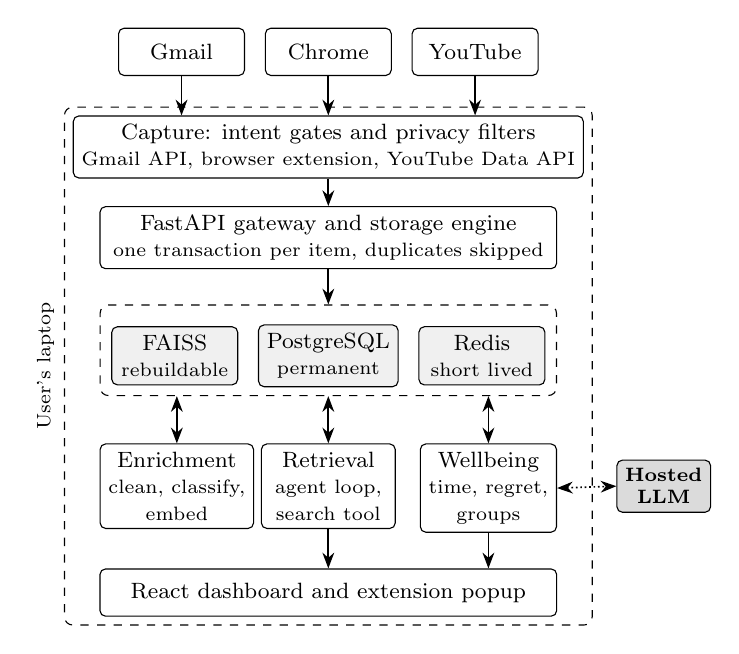
\begin{tikzpicture}[node distance=3.5mm and 2.5mm]
  \node[box, minimum width=16mm] (gm) {Gmail};
  \node[box, minimum width=16mm, right=of gm] (ch) {Chrome};
  \node[box, minimum width=16mm, right=of ch] (yt) {YouTube};
  \node[box, minimum width=58mm, below=5mm of ch] (cap)
      {Capture: intent gates and privacy filters\\ \scriptsize Gmail API, browser extension, YouTube Data API};
  \node[box, minimum width=58mm, below=of cap] (gw)
      {FastAPI gateway and storage engine\\ \scriptsize one transaction per item, duplicates skipped};
  \node[store, minimum width=16mm, below=7mm of gw] (pg) {PostgreSQL\\ \scriptsize permanent};
  \node[store, minimum width=16mm, left=of pg] (fa) {FAISS\\ \scriptsize rebuildable};
  \node[store, minimum width=16mm, right=of pg] (rd) {Redis\\ \scriptsize short lived};
  \node[grp, fit=(fa)(pg)(rd), inner ysep=5pt, yshift=2pt] (st) {};
  \node[box, minimum width=17mm, below=6mm of st.south west, anchor=north west] (enp)
      {Enrichment\\ \scriptsize clean, classify,\\ \scriptsize embed};
  \node[box, minimum width=17mm, below=6mm of st.south, anchor=north] (rse)
      {Retrieval\\ \scriptsize agent loop,\\ \scriptsize search tool};
  \node[box, minimum width=17mm, below=6mm of st.south east, anchor=north east] (wba)
      {Wellbeing\\ \scriptsize time, regret,\\ \scriptsize groups};
  \node[box, minimum width=58mm, below=5mm of rse] (ui) {React dashboard and extension popup};
  \node[grp, fit=(cap)(gw)(st)(enp)(wba)(ui), inner sep=3pt] (lap) {};
  \node[font=\scriptsize, rotate=90, anchor=south] at (lap.west) {User's laptop};
  \node[llm, minimum width=11mm, right=3mm of lap.east |- rse.east, anchor=west, font=\scriptsize\bfseries] (lm) {Hosted\\LLM};
  \draw[arr] (gm) -- (gm |- cap.north);
  \draw[arr] (ch) -- (cap);
  \draw[arr] (yt) -- (yt |- cap.north);
  \draw[arr] (cap) -- (gw);
  \draw[arr] (gw) -- (st.north);
  \draw[arr, {Stealth[length=2mm]}-{Stealth[length=2mm]}] (enp.north) -- (enp.north |- st.south);
  \draw[arr, {Stealth[length=2mm]}-{Stealth[length=2mm]}] (rse.north) -- (rse.north |- st.south);
  \draw[arr, {Stealth[length=2mm]}-{Stealth[length=2mm]}] (wba.north) -- (wba.north |- st.south);
  \draw[arr] (rse) -- (ui);
  \draw[arr] (wba.south) -- (wba.south |- ui.north);
  \draw[arr, densely dotted, {Stealth[length=2mm]}-{Stealth[length=2mm]}] (wba.east) -- (lm.west);
\end{tikzpicture}
\caption{The main parts of E.C.H.O. Everything inside the dashed frame runs on the user's laptop. The dotted arrow is the only path to the hosted language model of E.C.H.O; it carries bounded text from three callers (classification, retrieval, weekly reflection), described in Section~\ref{sec:privacy}.}
\label{fig:arch}
\end{figure}

% ---------------------------------------------------------------------
\section{Methodology}\label{sec:method}
% ---------------------------------------------------------------------
\subsection{Intent Aware Capture}
What should E.C.H.O keep? Each source has its own answer, and Table~\ref{tab:gates} summarizes them. These are the values we chose for the final system. The browser and the server hold matching copies, so that the server does not silently refuse a page that the extension sends.

Gmail is treated differently from the other two sources. Mail arrives on its own, so the user does not choose it. Also, few mails arrive each day, and even an unread message may matter later. So we store all messages when they arrive. The connector polls every 30 seconds, but each poll asks Gmail just for the changes since a saved history position. It does not list the entire mailbox each time. If that position has expired, the connector will list the mailbox once. Then the uniqueness rule on stored items absorbs the overlap. We do not read mail that Gmail has already filed as spam or trash, so Gmail's own spam filter also works as the spam filter of E.C.H.O. Whenever the user opens a message in Gmail on the web, the extension reports just the message id and the seconds spent reading.

For Chrome, a page is stored only after it clears a gate with two phases. In phase one, the page has to stay in the foreground for at least five seconds. If a page fails this phase, we drop it, and we remember only a page that passes it for revisit detection. Phase two comes next, where at least one sign of attention has to appear. This sign can be enough foreground time, enough scrolling, a real interaction, or a visit to the same page within the last 24 hours. Selecting text or clicking inside the page counts as an interaction, but clicking a link does not. This is because a click that leaves the page shows a choice to go elsewhere, and not interest in the page itself. We count time only while the tab is active, the window has focus, and the user has not been idle for 30 seconds. Along with the text of the main content, the extension also sends the top level headings of the page, so that the page can be found later by its topic.

We keep a YouTube video if the user watches it long enough, or watches a large enough share of it. Pausing, seeking, changing the speed, or returning to the same video within a day also keeps it. The completion rule needs at least five seconds of real watching, such that swiping past a short clip does not count as watching ten percent of it. Once a video has been watched for five seconds, the extension records the visit, so that a second short visit can pass through the revisit rule. Shorts are recognized by their page address, and they get a lower time bar, 10 seconds instead of 20, as the clips themselves are short.

\begin{table}[t]
\caption{Capture Rules for Each Source}
\label{tab:gates}
\centering
\renewcommand{\arraystretch}{1.05}
\begin{tabular}{|>{\raggedright\arraybackslash}p{1.35cm}|>{\raggedright\arraybackslash}p{6.2cm}|}
\hline
\textbf{Source} & \textbf{An item is kept when} \\
\hline
Gmail & Always, at arrival, except mail in Spam or Trash. Polled every 30~s for changes only. Reading time is added when a message is opened (opens under 3~s are ignored). \\
\hline
Chrome & Phase 1: at least 5~s in the foreground. Phase 2: any one of at least 10~s in the foreground, at least 15\% scroll depth, one interaction other than a link click, or a revisit within 24~hours. Work app pages: at least 5~s or one interaction, title only. \\
\hline
YouTube & Any one of at least 20~s of foreground playback (10~s for Shorts), at least 10\% of the video watched with at least 5~s of watching, a pause, seek, or speed change by the user, or a revisit within 24~hours. \\
\hline
\end{tabular}
\end{table}

\subsection{Storage Model}
Each email, page, and video gets one row in a central \texttt{memory\_items} table. What is specific to Gmail, Chrome, or YouTube goes into a matching source table, and attachments have their own table. Engagement counters such as reading time, watch time, and revisits change often, so they are kept apart from the item. Chrome and YouTube also add a row to a \texttt{visits} table for each admitted visit, with its time and the seconds spent. A page read on Monday and again on Thursday should count on both days, and one ``last seen'' time cannot show that. This is why the table exists. The schema has 17 tables.

A uniqueness rule on the pair of source type and source id keeps an item from being stored twice. This matters in practice. A connector can restart, or the Gmail connector may have to list the mailbox again, and in both cases it sends items we already have. Each item carries one of the five system groups, with misc as the fallback. New items are first written raw and flagged as unprocessed. We kept enrichment out of the capture path on purpose. It takes a few seconds per item, and capture should neither wait for that nor break when the worker crashes. When a revisited page comes back with different text, it gets flagged again and its vector is rebuilt. Timestamps are stored in UTC and shown in local time.

Deleting an item hides it from all queries. The user can also set a retention window of forever, one year, or six months. Forever is the default, since recalling old things is what the system is for. With a shorter window, a job at backend startup permanently removes the older items from PostgreSQL, the FAISS index, and Redis at the same time. All of them have to be cleaned together. If an item is removed from PostgreSQL but left in FAISS, it can still come back as a search hit.

\subsection{Background Enrichment}
A background worker picks up the unprocessed items every few seconds. It runs outside the capture path, so a slow step just delays the moment an item becomes searchable. Capture itself does not wait. Each item goes through four steps, and its final state is recorded at the end.

\textit{Cleaning.} For email, HTML is converted to text with the line breaks kept, and scripts, styles, tracking pixels, and hidden preview text are removed. When the sending app has split a body around an inline image, the parts are joined back together. Quoted earlier messages are removed, but the lines the sender typed between quoted lines are kept. This is because an inline reply is often the most important part of the message. A heuristic remover that we tested cut real body text in six of eight sample messages, while a leftover signature only adds a little noise. So signatures are deliberately left in place, as a little noise is better than lost body text. For a reply, keywords from earlier messages in the same thread are added, so that a terse ``Re:'' can still be found by its topic. For web pages, the extension has already picked the main content and the headings, and the worker separates the headings from the body. A video's text is made of its title, channel, category, tags, and description. The server also tries to download the caption text, but this is best effort, and it returned nothing for any of the 14 videos in our test data.

\textit{Attachments.} The same worker extracts attachment text when the mail is processed. It supports PDF, DOCX, XLSX, PPTX, HTML, forwarded messages, and plain text formats such as TXT, CSV, Markdown, JSON, and calendar files. Images and scanned PDFs are read with Tesseract OCR \cite{b15}, while inline images such as signature logos, and very small images, are skipped. The extracted text is stored next to the attachment record and not inside the email body. The beginning of each attachment joins the embedded text of the email, while the entire text joins the keyword index. So a line deep inside a file, say a clause in an offer letter or a date in a flight itinerary, can still be found by keyword. Both kinds of file are among the five PDFs in our test data.

\textit{Embedding.} We embed with the \embmodel{} sentence model \cite{b16}, which replaced \texttt{all-\allowbreak MiniLM-\allowbreak L6-\allowbreak v2} in our system. It reads at most 512 tokens and produces a 384 dimension vector. Since the window is fixed, the order of the text decides what gets lost when an item is too long. We put the short hints first: subject, keywords, and sender for mail, domain and headings for pages, and channel and category for videos. The long text, such as an email body or a description, goes last. If something has to be cut, it should be the end of a long body and not the subject or the sender, because those are what people tend to remember. The cut is made with the model's own tokenizer and ends at a whole word, and the text we store is exactly the text that was embedded. A mail with attachments gives its body up to 300 tokens, and the attachments get the rest. A video's description gets up to 200 tokens, and any caption text fills the remainder. The vector then goes into the FAISS index without a rebuild.

\textit{Classification.} Each item gets one of five broad groups: work, study, entertainment, personal, or misc. A cascade of four stages picks the group, and an item moves on to the next stage only if the current one cannot place it. Stage one uses structural signals from the source, such as Gmail category labels, academic mail domains, or the YouTube video category. Stage two looks the web domain up in a curated table. The idea of a cascade is that the cheap stages do most of the work, and on the 119 test items, that is what happened. Structural signals placed 84 items (70.6\%), the domain table 5 (4.2\%), and the group centers of stage three 11 (9.2\%). Only 19 (16.0\%) went to the language model.

Stage three compares the item's vector with a center for each group and accepts only a clear winner. A center starts as a seed, the mean of several example sentences written for its group. A seed has to lead the second best group by at least 0.05, a value we measured on labeled rows (Section~\ref{sec:eval}). After a group has ten confirmed items, its center is recomputed from them, with all sources weighted equally, so the center learns the topic instead of the look of one source. A recomputed center has to lead by at least 0.08, and both kinds of center need a cosine similarity of at least 0.55. Recomputation happens when the worker starts, if the stored centers are missing or older than 30 days. Stage four sends the language model one item at a time, with just its title and about 300 characters of text. With an OpenAI model this is a typed choice among the five group names. With other providers, the reply must be exactly one group name, and any other reply becomes misc. If the typed call fails, the item takes the single word path, so classification keeps going. We do not store a confidence value.

\textit{State tracking.} Each item ends up processed or failed. Failed items are set aside, neither counted as done nor lost, and a configuration switch lets the worker retry them.

\subsection{Retrieval Loop}
A question goes through the loop shown in Fig.~\ref{fig:graph}. The model, \llmname{}, receives the conversation so far, the question, one tool called \texttt{search\_memories}, and a small calendar around today's date, which takes the place of a separate date parser. The main argument of the tool is a query of a few keywords, and it comes with some options. These are up to two alternative phrasings, a list of sources, a start date, a reference item with the word before or after, and a flag to ask for attachment text. The model decides how to phrase the search. Then, in one round, it may issue several searches in parallel, for instance one per source. After reading the results, it either answers directly or searches again. On the first turn of a chat, the first call has to use the tool. A usual question needs one call that searches and one call that answers. The code allows at most five searches for one question, and at most three in one round. After the fifth search, we make the next call without the tool, such that the model has to answer. So a question costs between two and six model calls, and the program enforces this bound, not the prompt.

\begin{figure}[t]
\centering
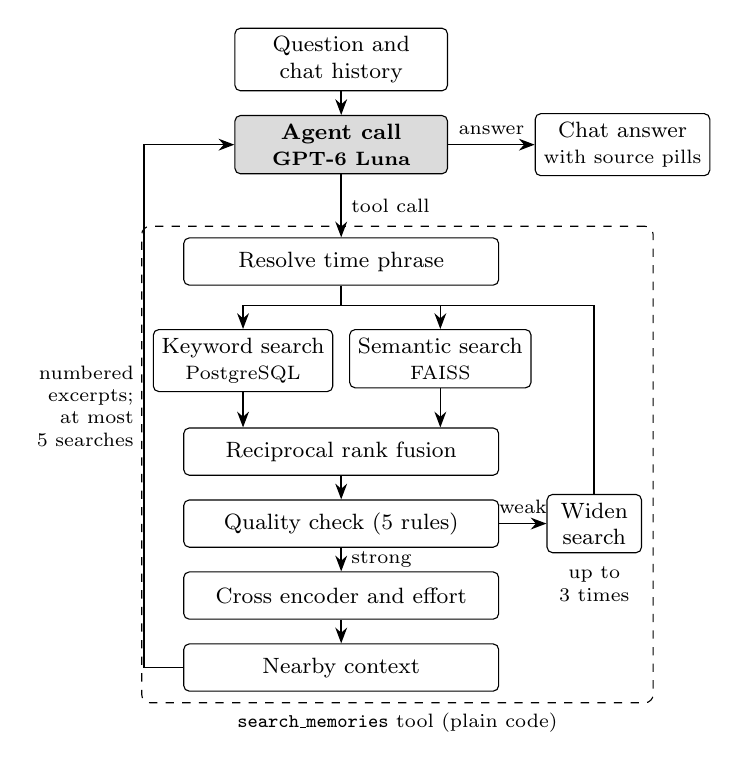
\begin{tikzpicture}[node distance=3mm and 3mm]
  \node[box, minimum width=27mm] (q) {Question and\\ chat history};
  \node[llm, minimum width=27mm, below=of q] (ag) {Agent call\\ \scriptsize\llmname};
  \node[box, minimum width=22mm, right=11mm of ag] (an) {Chat answer\\ \scriptsize with source pills};
  \node[box, minimum width=40mm, below=8mm of ag] (ta) {Resolve time phrase};
  \coordinate (bus) at ($(ta.south)+(0,-2.5mm)$);
  \node[box, minimum width=19mm, anchor=north east] (kw) at ($(bus)+(-1mm,-3mm)$) {Keyword search\\ \scriptsize PostgreSQL};
  \node[box, minimum width=19mm, anchor=north west] (se) at ($(bus)+(1mm,-3mm)$) {Semantic search\\ \scriptsize FAISS};
  \node[box, minimum width=40mm, anchor=north] (rrf) at ($(bus)+(0,-15.5mm)$) {Reciprocal rank fusion};
  \node[box, minimum width=40mm, below=of rrf] (qc) {Quality check (5 rules)};
  \node[box, minimum width=12mm, right=6mm of qc] (wd) {Widen\\search};
  \node[box, minimum width=40mm, below=of qc] (ce) {Cross encoder and effort};
  \node[box, minimum width=40mm, below=of ce] (nb) {Nearby context};
  \node[grp, fit=(ta)(kw)(se)(rrf)(qc)(wd)(ce)(nb), inner sep=4pt] (tool) {};
  \node[font=\scriptsize, anchor=north] at (tool.south) {\texttt{search\_memories} tool (plain code)};
  \draw[arr] (q) -- (ag);
  \draw[arr] (ag) -- node[above, font=\scriptsize] {answer} (an);
  \draw[arr] (ag) -- node[right, font=\scriptsize] {tool call} (ta);
  \draw[semithick] (ta.south) -- (bus);
  \draw[semithick] (bus -| kw.center) -- (bus -| wd.center);
  \draw[arr] (bus -| kw.center) -- (kw.north);
  \draw[arr] (bus -| se.center) -- (se.north);
  \draw[semithick] (wd.north) -- (wd.north |- bus);
  \node[font=\scriptsize, align=center, below=0.5mm of wd] {up to\\3 times};
  \draw[arr] (kw.south) -- (kw.south |- rrf.north);
  \draw[arr] (se.south) -- (se.south |- rrf.north);
  \draw[arr] (rrf) -- (qc);
  \draw[arr] (qc) -- node[above, font=\scriptsize] {weak} (wd);
  \draw[arr] (qc) -- node[right, font=\scriptsize] {strong} (ce);
  \draw[arr] (ce) -- (nb);
  \draw[arr] (nb.west) -- ++(-5mm,0) |- node[pos=0.25, left, font=\scriptsize, align=right] {numbered\\excerpts;\\at most\\5 searches} (ag.west);
\end{tikzpicture}
\caption{The retrieval loop. A language model gets called only in the shaded box. Everything inside the dashed frame is deterministic code, along with two small local encoders. When the search is widened, both search branches run again.}
\label{fig:graph}
\end{figure}

\textit{Resolve time phrase.} The model reads the calendar in its first message and passes a start date, so a phrase such as ``last Tuesday'' reaches the tool as a date. The tool accepts only a valid date. A phrase that points at another item, such as ``after the interview email,'' is passed as a reference item, and the code looks it up among the user's own items. The lookup tries keywords first and meaning second, with a minimum similarity. Once it finds the item, that item's time becomes a hard limit for both search branches. If no reference item is found, the search runs without that limit. An email counts as inside the range by its arrival time. A page or a video counts if any one of its recorded visits does. The date filter is open ended, so the answering call is told today's date and asked to use only the items inside the period the user named. Section~\ref{sec:eval} shows how our own test question of this kind, ``after the Brightwave interview email,'' turned out.

\textit{Parallel search.} Two branches search at once, in the same step of the graph. The semantic branch embeds the query and looks it up in FAISS. The keyword branch runs PostgreSQL full text search on a stored \texttt{search\_vector} column, which has a GIN index and holds the titles, the full text of each item, attachment text, senders, domains, and channel names. So a question about mail from one person can match on that person's name.

\textit{Fusion.} The two ranked lists are merged with reciprocal rank fusion \cite{b9}. For an item $d$, the fused score is
\begin{equation}
\mathrm{RRF}(d) = \sum_{b \in B} \frac{1}{k + r_b(d)}, \label{eq:rrf}
\end{equation}
where $B$ is the set of branches that returned $d$, $r_b(d)$ is its position in branch $b$ starting from 1, and $k = 60$. PostgreSQL's text rank and cosine similarity measure different things on different scales, so adding them would mean nothing, and working with positions avoids the problem. The top 50 fused items move on to the next step.

\textit{Quality check and widening.} Five rules decide whether the fused list is weak. It is weak if it is empty or holds fewer than two items, if none of its items comes from a source the user asked for, if none falls inside the time window, or if its best cosine similarity is below 0.55. This floor sits in a narrow gap. In the tests, the weakest answerable query still reached 0.558, and the best unanswerable one reached 0.573. At 0.55, none of the 38 answerable queries was flagged, but 2 of the 12 unanswerable ones got through (Section~\ref{sec:eval}). A weak list starts a wider search, and both branches run again. The first attempt stretches the time window by four days, opens all sources, or cuts the query to its core keyword. The second drops the time filter and the anchor. The third drops the keyword filters and searches a bigger part of the vector index. If all three fail, the tool reports that nothing was found, and the model can then tell the user so or try another phrasing.

\textit{Reranking.} The local cross encoder \rerankmodel{} \cite{b10}, \cite{b11} scores each remaining item against the question. It reads the title of the item followed by the beginning of its cleaned text, 512 characters in all. The final score blends this with an effort score:
\begin{equation}
s(d) = 0.8\,\sigma\big(c(q,d)\big) + 0.2\,e(d), \label{eq:final}
\end{equation}
where $c(q,d)$ is the cross encoder output for question $q$ and item $d$, $\sigma$ is the sigmoid function, and $e(d) \in [0,1]$ is the effort score. Effort is the mean of the engagement signals that an item has, such as reading or watch time, scroll depth, revisits, interactions, and how much of a video was watched. Each signal is capped and scaled to $[0,1]$. This favors the items that the user gave real attention to. Email is a special case. If a mail was read on a phone, or never opened in the browser, it has no measurable reading time. Instead of scoring such mail as zero, the reranker gives it the median effort of the other emails in the same result list. This way, an unmeasured email is neither punished nor promoted. By design, the score has no term for how recent an item is, and there is no diversity reranking.

\textit{Nearby context and excerpts.} The top three items bring their close neighbors with them, meaning other emails in the same thread, or pages and videos from the same browsing session or within five minutes. The model sees each result as a numbered entry. An entry has the title, source, and time, the sender, site, or channel, and the start of the cleaned text, capped at 8,000 characters for each of the top three and 2,000 for the rest. For a question about an attached file, the tool also adds the extracted text of the best ranked mail's attachment, up to 40,000 characters. This leaves plenty of room. The largest single request in the whole evaluation was 38,469 characters (Section~\ref{sec:eval}). The entry numbers stay fixed across all the searches for one question, so a citation always points to the same item.

\textit{Writing the answer.} The final call writes a conversational reply in Markdown. It gives the direct answer first, says plainly if something is missing, and asks back in one line if the question is ambiguous. Each fact carries a hidden marker that names the numbered item behind it. The backend keeps only markers that point to items that the tool actually returned, so the model cannot cite a source it did not see. On screen, each marker turns into a small pill with the sender, site, or channel and a short date, which is how people tend to remember an email anyway, by who sent it and roughly when. Clicking a pill then opens the original email, page, or video. Under the reply, a thin time strip also places the cited items on a timeline. While the loop is running, the dashboard shows progress messages, such as which source it is searching.

\textit{Failure handling.} If the model cannot be reached, the deterministic pipeline runs once on the raw question. In this case, the user still receives the ranked list of matching items, and not an error.

\subsection{Conversation Memory}
Each chat has a session id, and we save every turn in PostgreSQL on the laptop. When the user opens an old chat, its session picks up from where it was left. So a follow up such as ``show me Chrome pages about that topic after that email'' can refer back to an earlier answer. A new turn sends the model the last twelve messages, with each question cut to 1,000 characters and each answer to 3,000, so that a long old answer cannot take over the context meant for the new question. The citation numbers restart with every question. Chat history older than 30 days is deleted when the backend starts.

% ---------------------------------------------------------------------
\section{Wellbeing and User Groups}\label{sec:wba}
% ---------------------------------------------------------------------
The wellbeing module is built around one question: where did my time go? We gave the module one rule. It shows numbers and patterns, it gives the user no score, and nothing in it calls time wasted. Whether the time was well spent is for the user to decide.

\textit{Time.} Time totals are not stored anywhere. They are computed from the records when needed, so the same minutes cannot be counted twice. Page and video time comes from the \texttt{visits} table (Section~\ref{sec:method}), so each day gets exactly the time spent on it. Email time comes from the reading time the extension reports. Days are always the user's local days.

\textit{Sessions.} A session is a run of activity in which consecutive items are less than 20 minutes apart. We first planned a gap of 5 minutes, but a gap that short splits one sitting into two, so we moved to 20. This happens because each item is recorded at a single point in time. If the user reads a page for 15 minutes and then opens the next one, the record shows a 15 minute gap, even though the user was there the whole time. For each session, the module records how long it lasted, the system group that took the most time, and how many times the user switched between sources.

\textit{Regret.} Only the user decides what is regrettable, and any item can be marked. People change their minds, and we wanted to keep that history, so each mark and each unmark is stored as a new event instead of flipping a yes or no field. An item counts as regretted right now when it has an odd number of events. The module reports how many marked items fall in each content type and each hour. When the same kind of item is marked at a similar hour at least three times in 30 days, it flags that as a habit.

\textit{Weekly reflection.} Once a week, the module can write a short reflection. For this, one language model call receives only aggregated numbers, which are totals per category, regret counts, session patterns, and peak hours. It does not receive a title, an address, or any text from an item. Before the reply is shown, it is checked for judging phrases. If it fails this check, or if the call itself fails, a simple summary built from the same numbers is shown instead.

\textit{User groups.} System groups answer ``what kind of item is this?'', while user groups answer ``which of my goals does it serve?'', for example ``Placement prep.'' A user group starts with the items that the user files by hand. Once it has five confirmed items, an assignment job scores other items against it in two ways. The first way uses the rules the user wrote, each on a keyword, domain, channel, sender, or date range. The second way is a nearest neighbor score, which is the mean cosine similarity between the item and the three most similar confirmed members. An item is suggested when a rule matches, or when the neighbor score alone reaches a threshold. We set this threshold to 0.85, the lowest value at which no item outside a group scored at or above it in our test (Section~\ref{sec:eval}). The module can also propose a new rule when at least five confirmed members share a domain, sender, or channel.

When does E.C.H.O add something on its own? It does so only for a confident suggestion. A suggestion is confident if a rule matches and the neighbor score also reaches that same threshold. We add such an item directly, but the item still appears in the weekly review, where one click undoes it. So we handle confident items with a human on the loop. Anything less certain waits for an explicit accept in the review screen, which means the human stays in the loop. Also, an automatic addition does not count as a confirmed member until the user keeps it. So one wrong addition cannot pull in the next similar item. Manual filing and automatic additions pass through the same recorded path, so each membership has an audit trail. We never offer a rejected or removed suggestion again for that group. User groups are independent of the five system groups and have no parent among them, such that one goal can hold study pages and work mail together.

% ---------------------------------------------------------------------
\section{Privacy by Design}\label{sec:privacy}
% ---------------------------------------------------------------------
\textit{What is never captured.} Nothing from incognito windows is recorded, and the same goes for typed text and form input. Some pages also keep no text at all. A page falls in this case when its address contains a sensitive word, such as login, password, checkout, otp, or netbanking. Each word is matched as a whole word against a fixed list of 38. A page with a visible password box, or with a form of several personal fields, is treated the same way. Parameters that often carry secrets, such as tokens, one time codes, and session ids, are cut from every address before it is stored. Seven work apps, which are Slack, Atlassian, Notion, Figma, Linear, Trello, and Asana, are stored only as page titles and not as text. Their public help, blog, and documentation sections are still treated as ordinary pages. Gmail on the web is skipped by browser capture, because the mail already arrives through the Gmail API. All these lists live in one copy on the server, and the extension fetches them at startup. Until they arrive, the extension extracts no text.

\textit{What leaves the laptop.} The database, the vector index, the cache, and both encoders run locally. Two kinds of traffic leave the machine. First, requests to the Gmail and YouTube APIs fetch the user's own data. Second, calls to the hosted language model carry text from three callers. Retrieval sends the question, the recent chat history, and the numbered results. Each result is a title, a time, a sender, site, or channel, and the beginning of its text, at most 8,000 characters for each of the top three results and 2,000 for the others. When the user asks about a file, the text of one attachment is added, at most 40,000 characters. The classifier sends a title and about 300 characters, and it does so only for the items that the first three stages could not place. The weekly reflection sends only aggregated numbers. So a short email can reach the model whole, but a longer email, a page, or a transcript never does beyond these limits, and database rows and vectors are never sent. Requests to the hosted service are also subject to the data retention policy of its provider. Also, when the user connects an MCP client (Section~\ref{sec:impl}), the tool results go to that client, so its own language model sees the same excerpts.

\textit{Captured text is treated as data.} A newsletter or a web page can contain text written for a language model, such as ``ignore your previous instructions.'' This is known as prompt injection. In E.C.H.O, the worst such text can do is shape a search or an answer. It cannot delete or send anything. The only tool the model has is read only, and the system prompt tells the model that everything the tool returns is the user's data and not instructions. The retrieval logs record counts, scores, and timings, but not questions or titles.

\textit{User control.} The Settings page lets the user switch each source off and choose how long data is kept, and the extension popup has a switch that pauses capture. Domains and senders can also be excluded, single items can be deleted, and all the data can be exported as JSON or CSV. If the retention window is shorter than forever, old data is removed permanently.

% ---------------------------------------------------------------------
\section{Implementation}\label{sec:impl}
% ---------------------------------------------------------------------
The full stack is in Table~\ref{tab:stack}. We wrote the backend in Python and serve it with FastAPI. The retrieval loop is a LangGraph graph \cite{b5} in which an agent node and a tool node take turns under a round counter. All model calls go through LangChain, so changing the provider means changing one configuration entry, \texttt{LLM\_CONFIG} in \texttt{rse/config.py}. We relied on this during development, when we moved from Gemini to OpenAI by editing that entry. With OpenAI, the code also turns on features specific to it: the Responses API, medium reasoning effort for both retrieval calls, and the typed choice that the classifier uses. The embeddings and the cross encoder run locally on the CPU through the sentence transformers library. We built the dashboard with React and TypeScript, and the extension uses Chrome Manifest V3.

PostgreSQL 16 runs as a native service on the laptop, and Redis runs locally under the Windows Subsystem for Linux. So both stay on the laptop, and only standard HTTPS traffic leaves the machine.

E.C.H.O also runs as a server for the Model Context Protocol (MCP) \cite{b17}. Over the stdio transport, it exposes two read only tools, \texttt{search\_memories} and \texttt{get\_memory}. The first one has the same contract as the tool in the retrieval loop. So any MCP client, such as Claude Desktop, can query the memory with its own language model. In that case, the client plans the searches instead of the agent loop, while E.C.H.O stays the engine that does the actual searching.

\begin{table}[t]
\caption{Technology Used in the Final System}
\label{tab:stack}
\centering
\renewcommand{\arraystretch}{1.05}
\begin{tabular}{|>{\raggedright\arraybackslash}p{1.6cm}|>{\raggedright\arraybackslash}p{5.95cm}|}
\hline
\textbf{Layer} & \textbf{Technology} \\
\hline
Capture & Chrome extension (Manifest V3), Gmail API, YouTube Data API \\
\hline
Backend & Python, FastAPI, server sent events \\
\hline
Storage & PostgreSQL 16, FAISS, Redis, all local \\
\hline
Enrichment & Text extraction for PDF, DOCX, XLSX, PPTX, and EML; Tesseract OCR \\
\hline
Models & \embmodel{} embeddings (\embdim{} dimensions, 512 tokens),\newline \rerankmodel{} cross encoder,\newline \llmname{} through the OpenAI Responses API \\
\hline
Retrieval & LangGraph, LangChain, MCP Python SDK (stdio) \\
\hline
Interface & React, TypeScript, Vite \\
\hline
\end{tabular}
\end{table}

% ---------------------------------------------------------------------
\section{Evaluation}\label{sec:eval}
% ---------------------------------------------------------------------
\subsection{Setup}
We evaluated E.C.H.O on just one test account, which belongs to the authors. It holds 119 items, which are 78 emails, 30 pages, and 11 videos. Five of the emails carry a PDF attachment, and we extracted its text. We prepared 38 questions of five kinds. There are 16 about one item in one source, 4 about several sources, 6 with a time reference (``emails I received today,'' ``after the interview email''), 6 follow up questions that refer to an earlier turn, and 6 about the content of an attachment. Before the run, the relevant items for each question were marked. There are 81 of them in all, with at most eight for one question. We ran everything on one Windows laptop and called the hosted model through its API.

\subsection{Retrieval Quality}
We compare five configurations. The first four replay, for each question, the arguments that the model chose in its first search, so that they differ only in the stages of the tool. These are keyword search alone, semantic search alone, fusion without the cross encoder, and the full pipeline with quality check, widening, and reranking. The fifth is the whole agent loop. Table~\ref{tab:results} gives Recall@10, Recall@5, and the mean reciprocal rank (MRR) of the first relevant item within the first ten results. Recall@$k$ counts the relevant items among the first $k$ results and divides that by the smaller of $k$ and the number of relevant items.

\begin{table}[t]
\caption{Retrieval Quality on 38 Questions}
\label{tab:results}
\centering
\renewcommand{\arraystretch}{1.05}
\begin{tabular}{|l|c|c|c|}
\hline
\textbf{Configuration} & \textbf{R@10} & \textbf{R@5} & \textbf{MRR} \\
\hline
Keyword only & 0.697 & 0.697 & 0.693 \\
\hline
Semantic only & 0.955 & 0.934 & 0.987 \\
\hline
Fusion, no cross encoder & 0.955 & 0.934 & 0.987 \\
\hline
Full pipeline & 0.927 & 0.905 & 0.899 \\
\hline
Full agent loop & 0.927 & 0.905 & 0.899 \\
\hline
\end{tabular}
\end{table}

Keyword search alone reaches a recall of 0.70, because the full text search needs every query word to match, and for 11 of the 38 questions it found no relevant item. Semantic search alone and its fusion with keyword search both reach 0.955 with an MRR of 0.987. So on this collection, the keyword branch did not change the first ten results. Now the full pipeline scores lower. For five questions, the right item moved from first place to second or third place after reranking. In the two questions that we examined in detail, the cross encoder gave scores below 0.01 to all candidates. So the effort term of Eq.~\eqref{eq:final} decided the order, and an email that the user had opened outranked the right one. We therefore cannot claim that reranking helps on small collections of this kind.

The agent loop and the full pipeline have the same top ten, because later searches add items after the first ten. The loop pays off when we count everything it showed to the model. That was 70 of the 81 relevant items, against 65 for a single pass (0.86 against 0.80), at the cost of showing more results. The gain came from three questions in which a second search found items that the first one missed. Split by kind, the loop's recall was 1.00 for single source, follow up, and attachment questions. It fell to 0.74 for questions over several sources and to 0.71 for questions with a time reference. Part of the time loss comes from the open date filter. If a question gives just a start date, there is no end date, and later items crowd into its results. In the question ``after the Brightwave interview email,'' the model wrote the phrase into the query and did not use the reference item, which gave a recall of 0.20. The answers to all 11 questions whose answer contains a unique fact were correct.

\subsection{Cost and Speed}
The 38 questions made 44 turns, since each follow up has two. A turn needed 2.34 model calls on average. In detail, 33 turns used two calls, 8 used three, 2 used four, and 1 used five. No turn used all five searches. Four was the most. The median response time was 8.1 seconds, the 95th percentile was 23.8 seconds, and the longest was 30.2 seconds. On average, a turn sent 8,983 input tokens and received 238 output tokens. At an assumed price of 0.20 and 1.20 US dollars per million input and output tokens, this comes to about 0.002 dollars per turn.

\subsection{Capture Accuracy}
We replayed 15 scripted browsing and viewing sessions in a test profile of Chrome with the extension. The sessions include a page closed after three seconds, a page read for six seconds without scrolling, a page scrolled to 20 percent, a click on a link, and a text selection. They also include a page address with a secret parameter, a video closed after three seconds, a ten minute video watched for seven seconds twice, and a video watched for 25 seconds. Before the run, we wrote down the expected result of each session from the rules. Thirteen sessions were clean, and in all 13 the stored items matched the rules (8 Chrome and 5 YouTube sessions). Two further sessions were discarded because a person used the browser during them. A script drove the sessions and also kept the system from going idle, and the durations are accurate to about two seconds.

\subsection{Privacy Audit}
During the evaluation, we recorded all requests to the language model. The largest request held 38,469 characters. Two items in the collection are longer than the 8,000 character limit for the top results, and both were shown to the model. The text beyond the limit appeared in no request.

\subsection{Threshold Calibration}
Three similarity cutoffs depend on the embedding model, so we measured them on the collection. First, we looked at the seed centers of classification stage three. We took the 78 items whose group was already known from structural signals. A lead of 0.08 did not fire even once on them, while a lead of 0.05 fired 14 times, and all 14 were correct. No item scored below 0.585, so the 0.55 floor could not be tested at all. Second, we looked at the quality check. The best cosine similarity of the 38 answerable queries did not drop below 0.558, and its median was 0.734. The 12 unanswerable queries reached at most 0.573. A floor of 0.55 flags none of the good queries and lets 2 of the 12 bad ones through. Raising it to 0.58 would stop those 2 but wrongly flag 1 good query, and with a single query deciding it, we had no real evidence to move, so we kept 0.55. Third, we looked at the nearest neighbor score for user groups. We formed three groups of 13, 5, and 5 items, scored each member against the rest of its group, and scored all the other items against each group. At 0.65, all 23 members pass, but so do 155 of the 358 other items. At 0.85, 7 members pass and no other item does, which makes 0.85 the lowest value with no wrong item, and that is the value we use. This choice has a cost. On meaning alone, only about 30\% of true members reach 0.85, so most suggestions will come from the user's rules and not from similarity. The groups and their labels are provisional, and the sample is small.

Placeholder paragraph two of the threshold section.

Placeholder paragraph three of the threshold section.

% ---------------------------------------------------------------------
\section{Limitations and Future Work}\label{sec:limits}
% ---------------------------------------------------------------------
Coverage is the biggest limit. E.C.H.O sees only desktop Chrome, so anything done on a phone is missing. YouTube history starts on the day the extension is installed, and playback in the background or in picture in picture mode is not tracked. Each item has just one vector, so for a long document only the first 512 tokens shape its meaning based match, and anything deeper can be reached only by keyword. Outlook replies quote the older thread without a marker that E.C.H.O removes, so such threads can show up more than once. The date filter has no end, and only the top ten results of each search reach the answering call, so on a busy day a question about yesterday can get crowded out by today's items. Classification also has a weak spot. Stage one trusts Gmail's own labels. In our data, Gmail had labeled an offer letter and a course syllabus as Personal, so E.C.H.O filed both as personal too. Pages from private apps outside the seven listed, such as chat assistants or online documents, are captured like ordinary pages unless the user excludes their domain. The OAuth tokens are plain files, protected only by the file permissions of the operating system. Captions are fetched on a best effort basis, and none came back for our videos, so a video's text rests on its title, tags, and description.

The evaluation is also narrow. It uses one account with 119 items and 38 questions prepared within the project, not by independent users. One question moves a recall figure by about 2.6 percentage points, so the results may not carry over to larger collections or to other users. One of those questions also showed a weakness in how the model uses the tool. For ``after the Brightwave interview email,'' it put the phrase into the query instead of passing the reference item, and it lost relevant items as a result. Tesseract was not installed in our test setup, so we could not evaluate scanned files. The wellbeing module and the group suggestions were not tested with users. Finally, the language model is a hosted service, so its availability and its limits apply.

Reranking comes first, since that is where our results hurt the most. In our test, the weight on engagement outweighed relevance and lowered MRR from 0.987 to 0.899. Then comes a larger evaluation over several users, with questions written by people who did not build the system. We also plan to store several vectors for each long item and to let the domain table learn from labels that the user confirms. Importing past history from Google Takeout and from the browser's own history file would also let a new user start with a full memory instead of an empty one.

% ---------------------------------------------------------------------
\section{Conclusion}\label{sec:conc}
% ---------------------------------------------------------------------
E.C.H.O turns a person's email, browsing, and video history into one memory they can ask questions of. It keeps all legitimate mail but only the pages and videos that got the user's attention, stores everything on the user's laptop, and prepares it for search in the background. The language model plans each search and plain code runs it, which keeps the model's role visible, its calls bounded, and its cost low, while the wellbeing module describes time and leaves the user in charge of every personal group. On 119 items, a question needed 2.3 model calls and a median of 8.1 seconds, and the first ten results held 93\% of the relevant items. The main lesson for us came from what did not work. On a small personal collection, a good small embedding model did most of the ranking, the cross encoder did not improve on it, and the model did not always use a reference to another item. Where the agent loop did help was recall across several searches, as it showed the model 0.86 of the relevant items against 0.80 for a single pass.

\section*{Acknowledgment}
We thank the Department of Computer Science and Engineering, PES University, for supporting this capstone project, and the faculty who reviewed our work at each phase for their questions and feedback.

\IEEEtriggeratref{99}
\begin{thebibliography}{00}
\bibitem{b1} V. Bush, ``As we may think,'' \textit{The Atlantic Monthly}, vol. 176, no. 1, pp. 101--108, Jul. 1945.
\bibitem{b2} S. Dumais, E. Cutrell, J. J. Cadiz, G. Jancke, R. Sarin, and D. C. Robbins, ``Stuff I've seen: A system for personal information retrieval and re-use,'' in \textit{Proc. 26th Annu. Int. ACM SIGIR Conf. Research and Development in Information Retrieval}, Toronto, Canada, 2003, pp. 72--79.
\bibitem{b3} J. Gemmell, G. Bell, and R. Lueder, ``MyLifeBits: A personal database for everything,'' \textit{Commun. ACM}, vol. 49, no. 1, pp. 88--95, Jan. 2006.
\bibitem{b4} P. Lewis, E. Perez, A. Piktus, F. Petroni, V. Karpukhin, N. Goyal, H. K\"{u}ttler, M. Lewis, W. Yih, T. Rockt\"{a}schel, S. Riedel, and D. Kiela, ``Retrieval-augmented generation for knowledge-intensive NLP tasks,'' in \textit{Advances in Neural Information Processing Systems}, vol. 33, 2020, pp. 9459--9474.
\bibitem{b5} LangChain, ``LangGraph,'' GitHub repository. [Online]. Available: \url{https://github.com/langchain-ai/langgraph} (accessed Oct. 21, 2026).
\bibitem{b13} S. Yao, J. Zhao, D. Yu, N. Du, I. Shafran, K. Narasimhan, and Y. Cao, ``ReAct: Synergizing reasoning and acting in language models,'' in \textit{Proc. 11th Int. Conf. Learning Representations (ICLR)}, Kigali, Rwanda, 2023.
\bibitem{b6} N. Reimers and I. Gurevych, ``Sentence-BERT: Sentence embeddings using Siamese BERT-networks,'' in \textit{Proc. 2019 Conf. Empirical Methods in Natural Language Processing and 9th Int. Joint Conf. Natural Language Processing (EMNLP-IJCNLP)}, Hong Kong, China, 2019, pp. 3982--3992.
\bibitem{b16} L. Merrick, D. Xu, G. Nuti, and D. Campos, ``Arctic-Embed: Scalable, efficient, and accurate text embedding models,'' arXiv:2405.05374, 2024.
\bibitem{b8} J. Johnson, M. Douze, and H. J\'{e}gou, ``Billion-scale similarity search with GPUs,'' \textit{IEEE Trans. Big Data}, vol. 7, no. 3, pp. 535--547, Jul. 2021.
\bibitem{b9} G. V. Cormack, C. L. A. Clarke, and S. B\"{u}ttcher, ``Reciprocal rank fusion outperforms Condorcet and individual rank learning methods,'' in \textit{Proc. 32nd Int. ACM SIGIR Conf. Research and Development in Information Retrieval}, Boston, MA, USA, 2009, pp. 758--759.
\bibitem{b10} R. Nogueira and K. Cho, ``Passage re-ranking with BERT,'' arXiv:1901.04085, 2019.
\bibitem{b7} W. Wang, F. Wei, L. Dong, H. Bao, N. Yang, and M. Zhou, ``MiniLM: Deep self-attention distillation for task-agnostic compression of pre-trained transformers,'' in \textit{Advances in Neural Information Processing Systems}, vol. 33, 2020, pp. 5776--5788.
\bibitem{b11} P. Bajaj \textit{et al.}, ``MS MARCO: A human generated machine reading comprehension dataset,'' arXiv:1611.09268, 2016.
\bibitem{b12} M. Kleppmann, A. Wiggins, P. van Hardenberg, and M. McGranaghan, ``Local-first software: You own your data, in spite of the cloud,'' in \textit{Proc. ACM SIGPLAN Int. Symp. New Ideas, New Paradigms, and Reflections on Programming and Software (Onward!)}, 2019, pp. 154--178.
\bibitem{b14} U. Lyngs \textit{et al.}, ``Self-control in cyberspace: Applying dual systems theory to a review of digital self-control tools,'' in \textit{Proc. CHI Conf. Human Factors in Computing Systems (CHI '19)}, Glasgow, UK, 2019, doi: 10.1145/3290605.3300361.
\bibitem{b15} R. Smith, ``An overview of the Tesseract OCR engine,'' in \textit{Proc. 9th Int. Conf. Document Analysis and Recognition (ICDAR)}, Curitiba, Brazil, 2007, pp. 629--633.
\bibitem{b17} Model Context Protocol, ``Model Context Protocol specification.'' [Online]. Available: \url{https://modelcontextprotocol.io/} (accessed Oct. 26, 2026).
\end{thebibliography}

\end{document}
